\documentclass[11pt,a4paper]{article}

\usepackage{fontspec}
\usepackage[russian]{babel}
\setmainfont{cmunrm.otf}[BoldFont=cmunbx.otf,ItalicFont=cmunti.otf,BoldItalicFont=cmunbi.otf]
\setsansfont{cmunss.otf}[BoldFont=cmunsx.otf,ItalicFont=cmunsi.otf,BoldItalicFont=cmunso.otf]
\setmonofont{cmuntt.otf}[BoldFont=cmuntb.otf,ItalicFont=cmunit.otf,BoldItalicFont=cmuntx.otf]

\usepackage[left=20mm,right=15mm,top=18mm,bottom=20mm]{geometry}
\usepackage{amsmath}
\usepackage{graphicx}
\usepackage{float}
\usepackage{xcolor}
\usepackage{booktabs}
\usepackage{tabularx}
\usepackage{array}
\usepackage{listings}
\usepackage[most]{tcolorbox}
\usepackage[labelsep=period,font=small,skip=3pt]{caption}
\usepackage{enumitem}
\usepackage{xurl}
\usepackage[hidelinks,pdfauthor={Тищенко П. В.},pdftitle={MapReduce и DuckDB на RustFS: навыки и зарплаты PHP-разработчиков}]{hyperref}

\definecolor{accent}{HTML}{2F5D9C}
\definecolor{ok}{HTML}{1E7A45}
\definecolor{bad}{HTML}{B3261E}
\definecolor{codebg}{HTML}{F4F5F8}
\definecolor{cmt}{HTML}{6B7280}

\setlength{\parindent}{1cm}
\setlength{\emergencystretch}{3em}
\setlist{itemsep=1pt,topsep=3pt}
\renewcommand{\arraystretch}{1.15}
\newcolumntype{L}{>{\raggedright\arraybackslash}X}
\setlength{\abovecaptionskip}{3pt}
\setlength{\intextsep}{6pt}

\lstset{
  basicstyle=\ttfamily\scriptsize,
  columns=fixed,
  basewidth=0.525em,
  keepspaces=true,
  breaklines=true,
  backgroundcolor=\color{codebg},
  frame=leftline,
  rulecolor=\color{accent},
  framerule=1.5pt,
  xleftmargin=6pt,
  framexleftmargin=4pt,
  aboveskip=4pt,
  belowskip=6pt,
  showstringspaces=false,
  extendedchars=true,
  moredelim=[is][\color{bad}\bfseries]{@@}{@@},
  moredelim=[is][\color{ok}\bfseries]{++}{++},
  moredelim=[is][\color{cmt}]{~~}{~~}
}

\newcommand{\code}[1]{\texttt{#1}}
\newtcolorbox{keybox}{enhanced,breakable,colback=accent!6,colframe=accent,boxrule=0.6pt,arc=0pt,left=5pt,right=5pt,top=3pt,bottom=3pt,before upper={\setlength{\parindent}{0pt}}}

\begin{document}

\begin{titlepage}
  \centering
  \vspace*{15mm}
  {\large Домашнее задание №\,3\par}
  {\large «Технология MapReduce»\par}
  \vspace{40mm}
  {\LARGE\bfseries Свой MapReduce и DuckDB\\[4pt] поверх объектного хранилища RustFS\par}
  \vspace{8mm}
  {\normalsize Частоты навыков, пар и троек, зарплаты и регионы\\ Вариант 5: «Программист, разработчик на PHP»\par}
  \vfill
  \begin{flushright}
    \begin{tabular}{@{}l@{}}
      Выполнил: \textbf{Тищенко Павел Валерьевич}\\
      Группа ИИИ-3-ИнжДан-1-1 (J3310), №\,16\\
      Репозиторий: \url{https://github.com/paulhowever/vk_data_eng_2026_ai_67_tischenko}
    \end{tabular}
  \end{flushright}
  \vspace{25mm}
  {2026\par}
\end{titlepage}

\section{Стенд, хранилище и данные}

\begin{table}[H]
\centering
\small
\caption{Стенд}
\begin{tabularx}{\linewidth}{@{}lL@{}}
\toprule
Машина & Apple M5, 10 ядер, 16 ГБ RAM, macOS; Docker Engine 29.2; Python 3.13, uv \\
Хранилище & RustFS 1.0.0, 4 диска \code{.data/disk1..4} (EC 2+2), S3 API \code{localhost:19000}, консоль \code{:19001} \\
Объект & \code{s3://hh-lake/raw/it\_vacancies\_2024.csv} --- 847\,619\,384 Б, 229\,388 вакансий hh.ru за 2024 г. \\
Вариант & \code{role = 'Программист, разработчик' AND name ILIKE '\%php\%'} --- 5\,382 вакансии, 4\,380 с навыками \\
Навыки & split по \code{;} $\to$ trim $\to$ lower $\to$ без пустых $\to$ distinct в вакансии; синонимы (php7/php8, js/javascript) не склеиваются \\
\bottomrule
\end{tabularx}
\end{table}

Хранилище поднято из \code{docker-compose.yml} (как в ДЗ\,2, порты сдвинуты на 19000/19001), объект загружен скриптом \code{hhlake.upload}; целостность проверена по sha256 потока из S3 (ETag multipart-загрузки --- не MD5):
\begin{lstlisting}
$ uv run python -m hhlake.upload
uploaded /Users/paveltischenko/Downloads/it_vacancies_2024.csv -> s3://hh-lake/raw/it_vacancies_2024.csv
remote size  847,619,384 B  etag "0e6d21890db664d9bf83e1427665b106-13"
sha256 local  303db922b541e4440906f5a7e8be32fb55e8808f950ffddb8c272f1548212a65
sha256 remote 303db922b541e4440906f5a7e8be32fb55e8808f950ffddb8c272f1548212a65
++integrity     OK++
\end{lstlisting}

\begin{figure}[H]
  \centering
  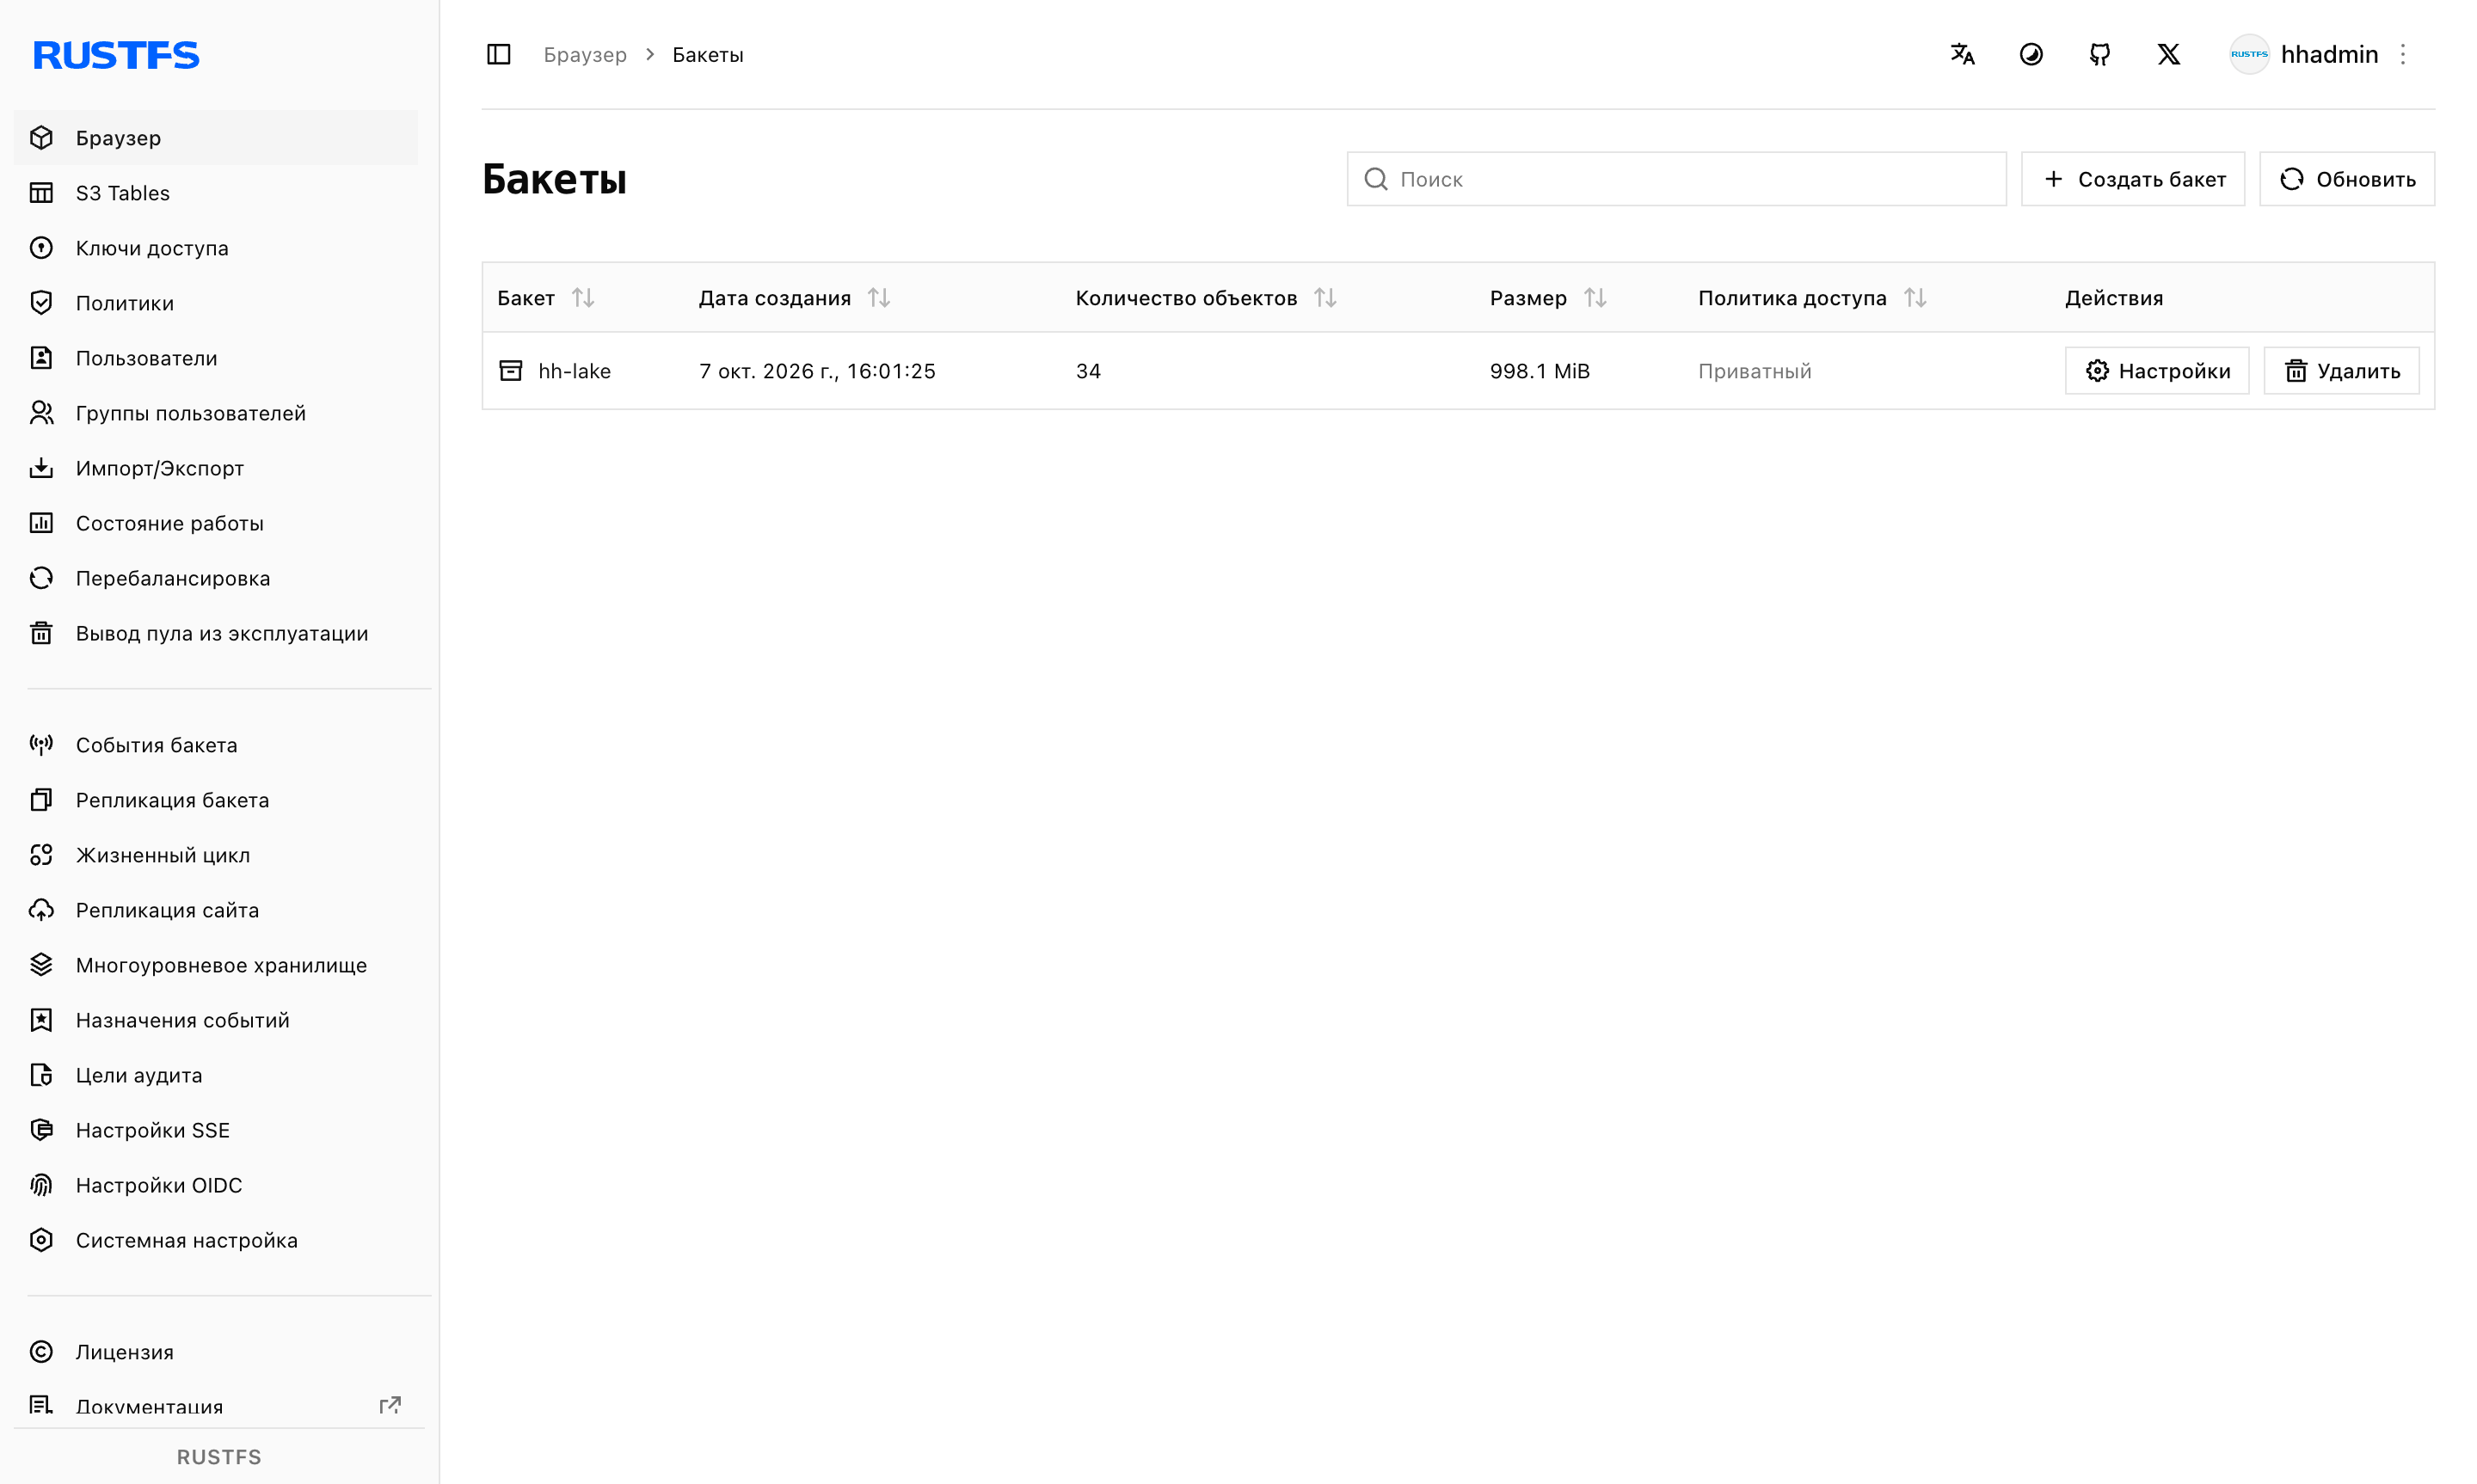
\includegraphics[width=0.49\linewidth]{img/console_buckets.png}\hfill
  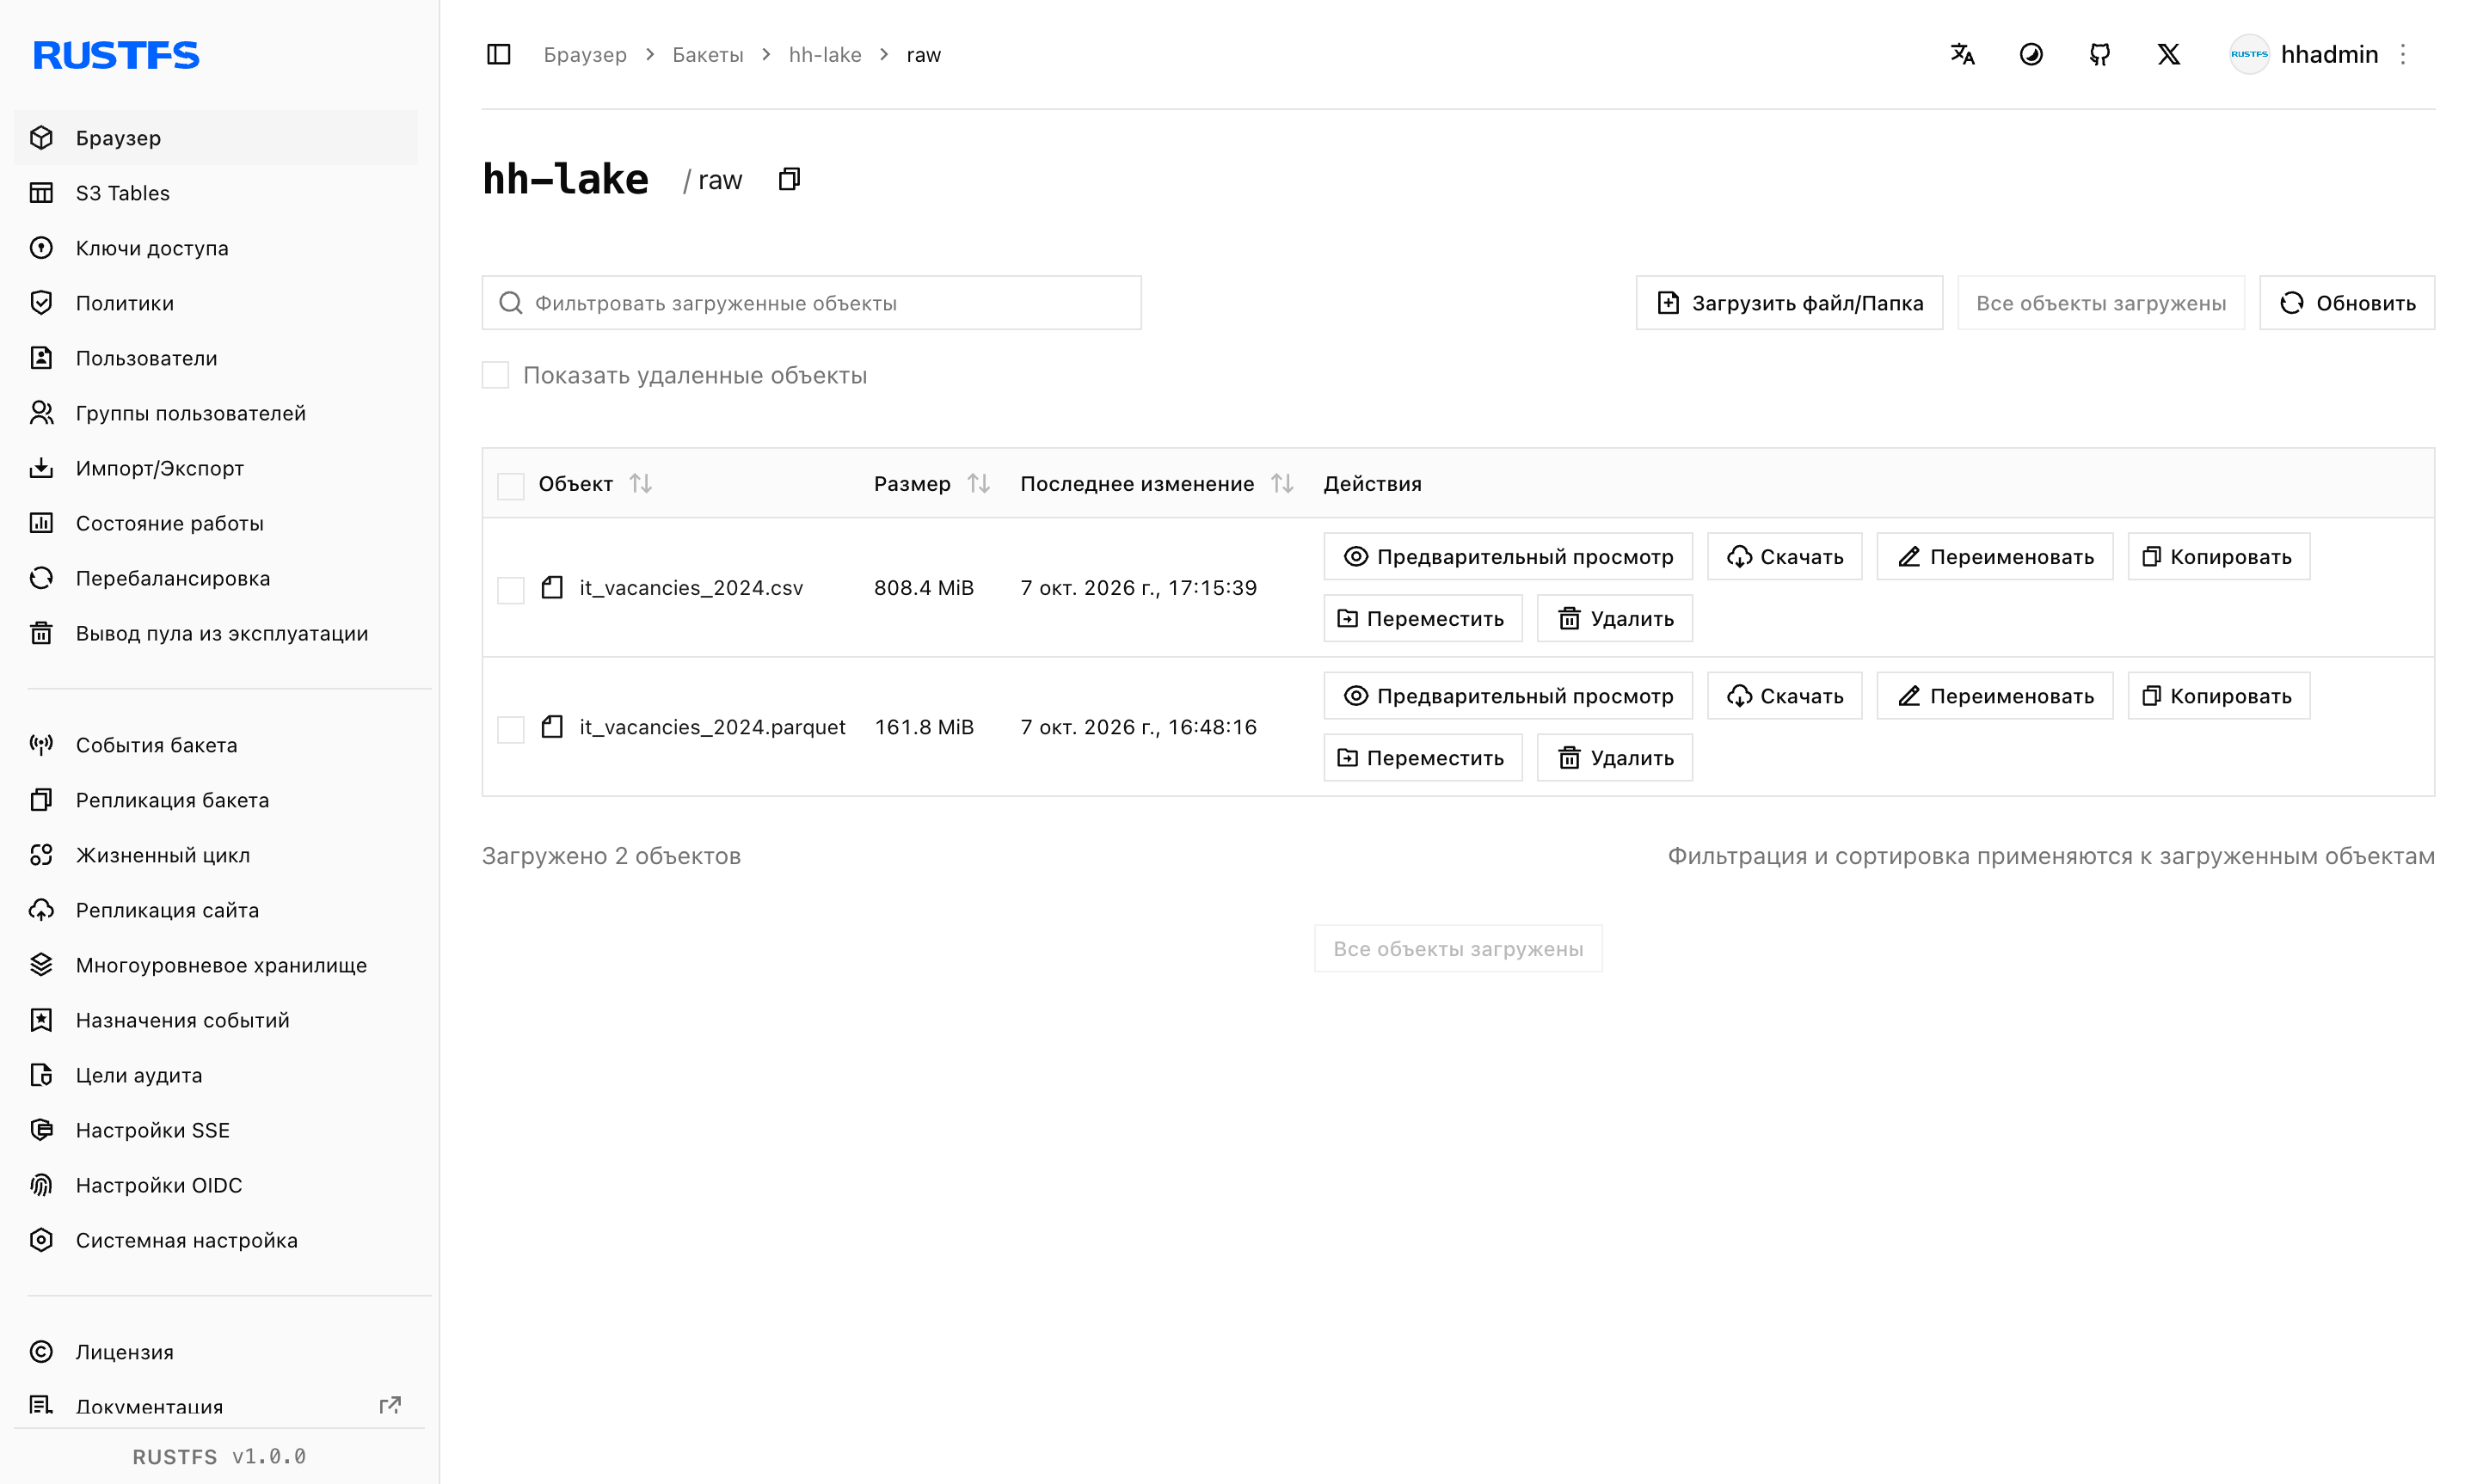
\includegraphics[width=0.49\linewidth]{img/console_raw.png}
  \caption{Консоль RustFS: бакет \code{hh-lake} (34 объекта, 998 МиБ) и \code{raw/} с исходным CSV и Parquet-копией}
\end{figure}

\section{Собственный MapReduce из S3}

Реализация --- пакет \code{hhlake.mr} (\code{split.py}, \code{jobs.py}, \code{engine.py}, \code{run.py}). Данные читаются только из S3, локальный путь в коде вычислений не используется.
\begin{itemize}
  \item \textbf{Split.} Объект делится на чанки по 32 МиБ (26 map-задач). Каждый маппер делает один Range GET \code{bytes=(start-1)..(end+64\,КиБ)} и при необходимости докачивает хвост. Запись принадлежит мапперу, в чей диапазон попал её первый байт; граница --- регулярное выражение \code{\textbackslash n(?=hh,\textbackslash d+,)} со строгой проверкой записи (23 поля, статус, дата, ссылка вида \code{hh.ru/vacancy/<id>}); UTF-8 декодируется только после выравнивания. Корректность на «злом» файле (переводы строк и ложные префиксы внутри кавычек) покрыта \code{tests/test\_split.py}.
  \item \textbf{Map + combiner.} \code{csv.reader} $\to$ условие варианта $\to$ нормализация $\to$ сочетания \code{combinations(skills, k)} для $k=1,2,3$ за один проход $\to$ \code{Counter} внутри маппера.
  \item \textbf{Shuffle.} Партиция \code{crc32("\textbackslash t".join(key)) \% R} (не \code{hash()}: в spawn-процессах соль разная). Каждая попытка маппера пишет свои партиции в S3 под отдельным префиксом \code{tmp/mr/<job>/map-<i>-a<n>/}.
  \item \textbf{Reduce.} 4 редьюсера читают партиции только успешных попыток из \code{\_manifest.json}, мастер сортирует и пишет \code{results/mapreduce/k\{1,2,3\}.csv}.
  \item \textbf{Мастер.} \code{ProcessPoolExecutor}: при падении процесса ловит \code{BrokenProcessPool}, пересоздаёт пул и перезапускает незавершённые задачи (до 3 попыток).
\end{itemize}

\begin{lstlisting}
$ uv run python -m hhlake.mr.run --k 1 2 3
chunk 32 MiB  workers 10  reducers 4
map    task   0  attempt 1  ok   pid 15318  2.12 s  bytes [222, 33,555,287)  records 8,969  GET 1
...                                                     ~~(26 map-задач)~~
reduce task   0  attempt 1  ok   pid 15317  0.20 s  parts 26  bytes 4,522,383  keys 36,138
map 5.78 s   reduce 0.24 s   map tasks 26
S3 input: 27 GET, 849,323,345 B (+1,703,961 B vs object)
S3 shuffle: 104 PUT, 104 GET, 18,080,028 B
  fetch: Range GET + record alignment                   33.62 s  72.7%
  parse: UTF-8 decode + csv.reader                       2.72 s   5.9%
  combine: filter, normalize, combinations, Counter      0.40 s   0.9%
  put: shuffle PUT to S3                                 8.94 s  19.3%
++ok   records 229,388   unique vacancy_id 229,388   variant 5,382   with skills 4,380++
\end{lstlisting}

\begin{figure}[H]
  \centering
  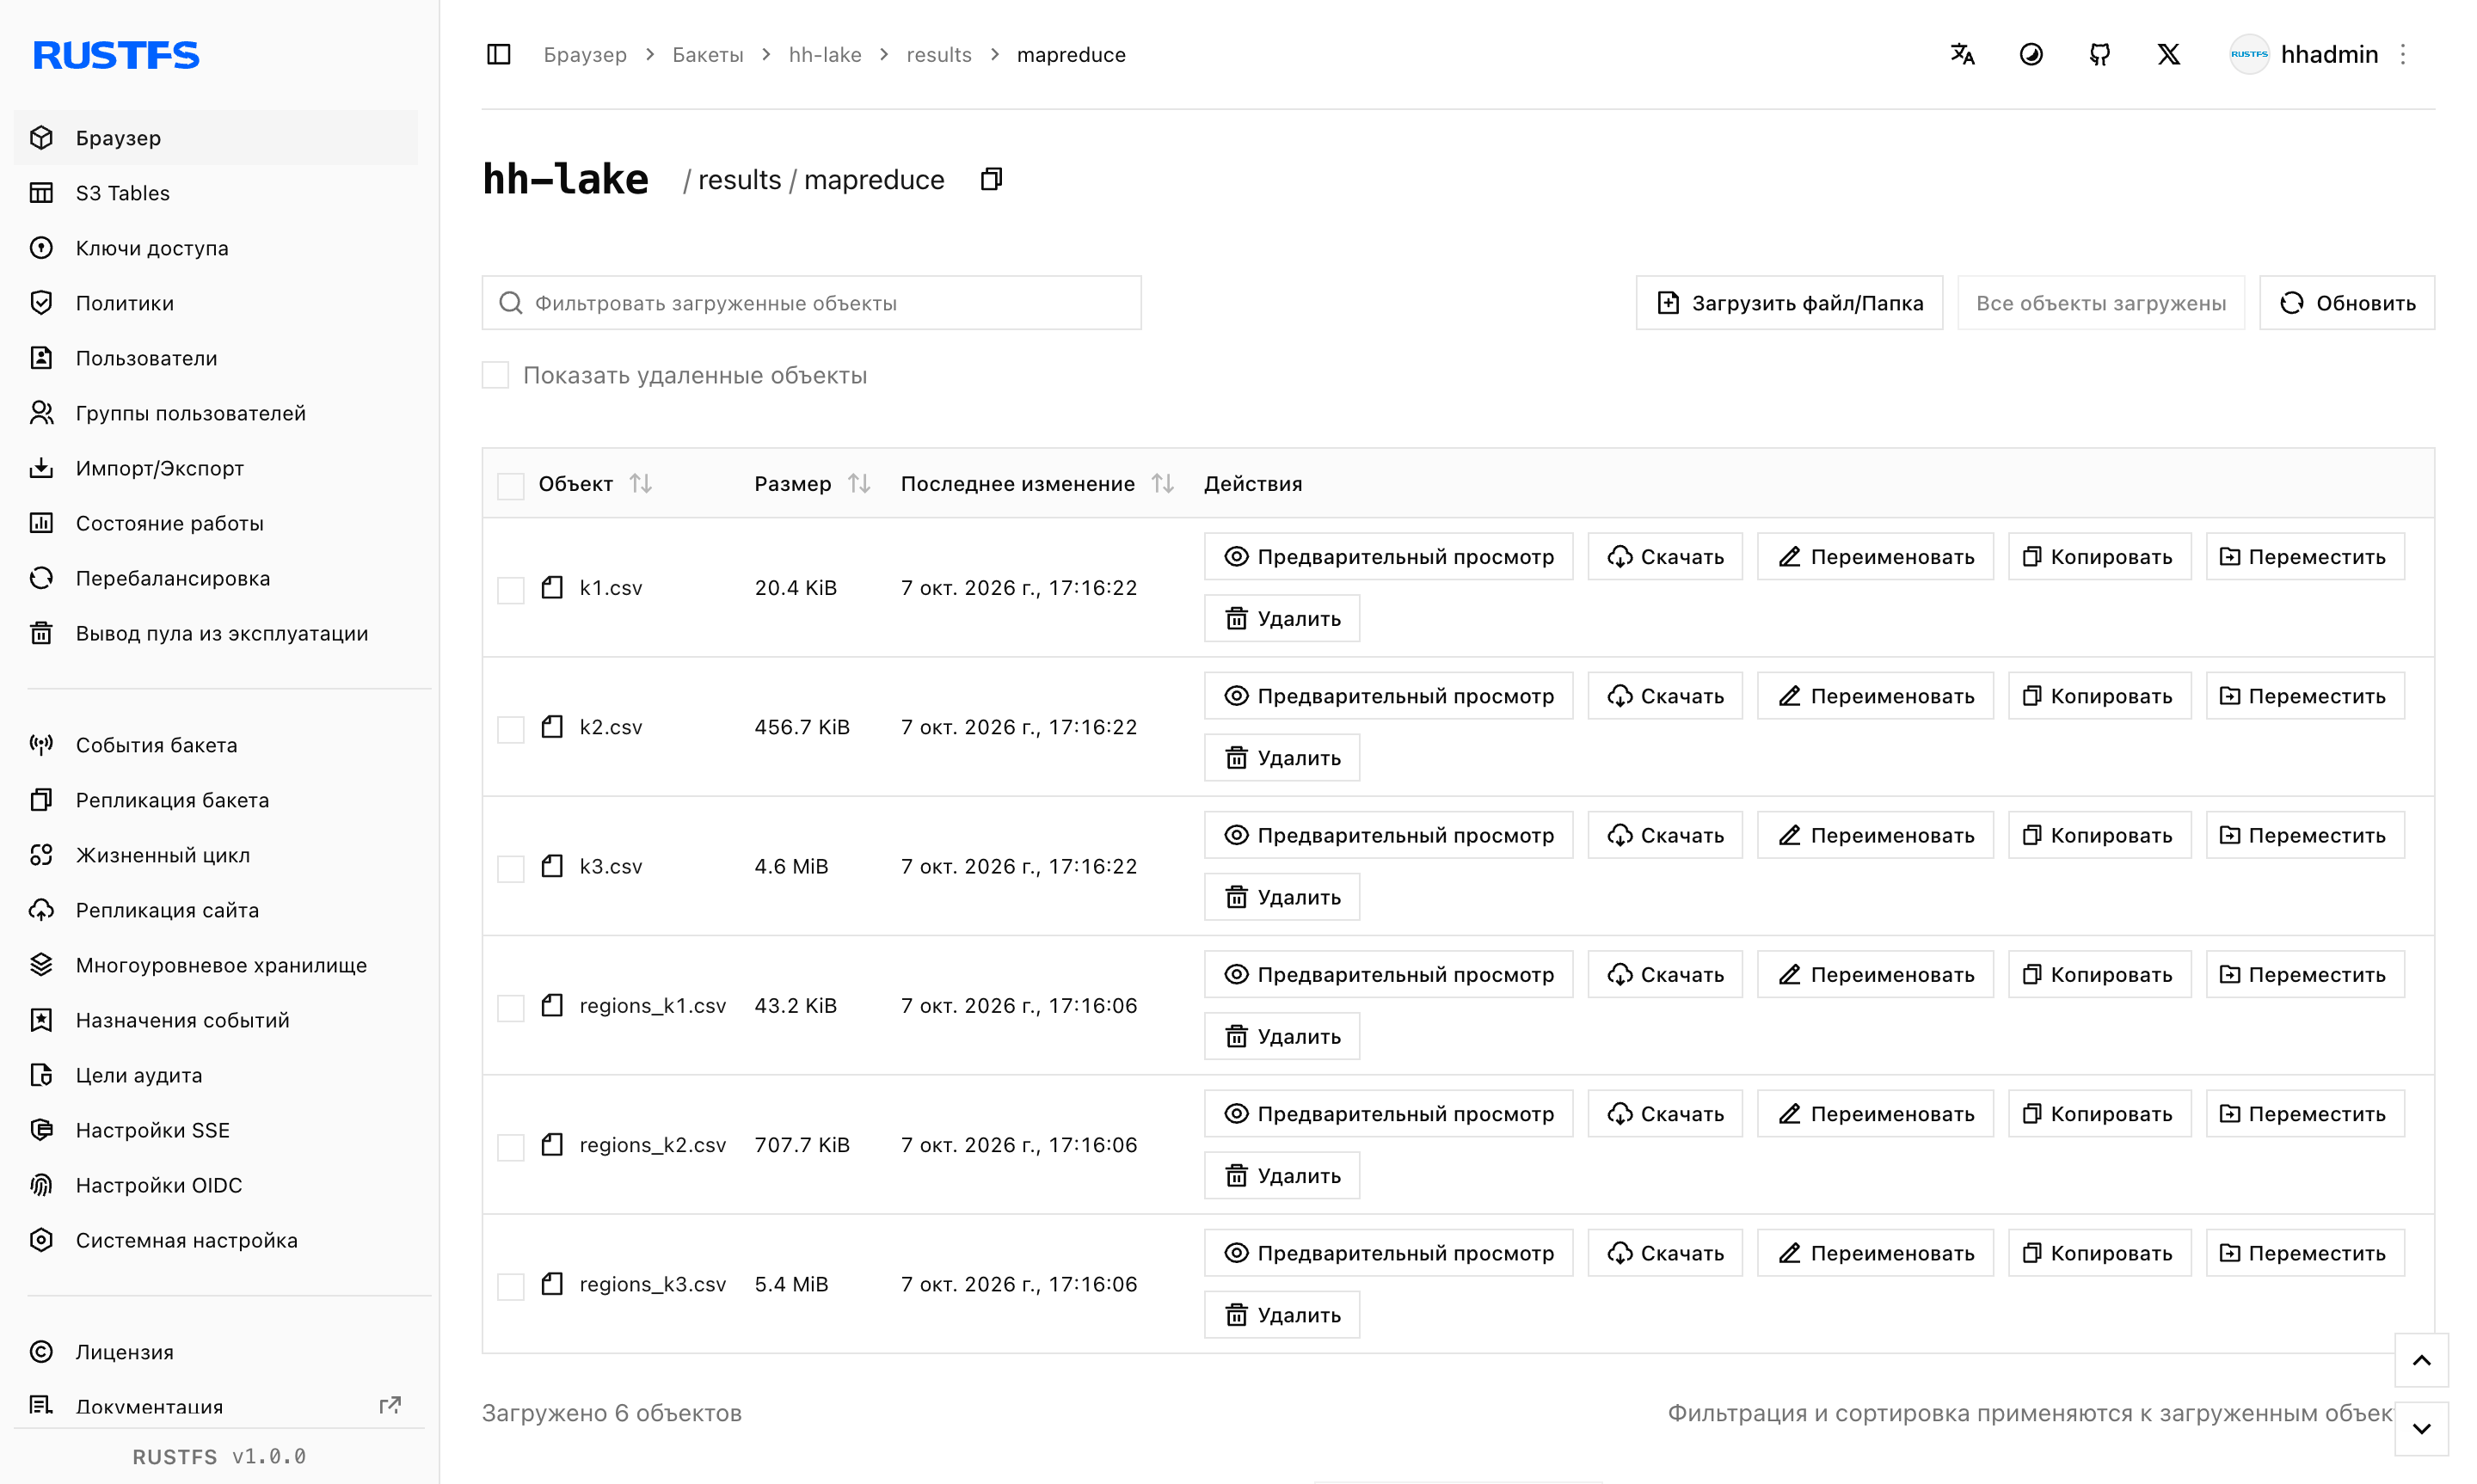
\includegraphics[width=0.49\linewidth]{img/console_mr.png}\hfill
  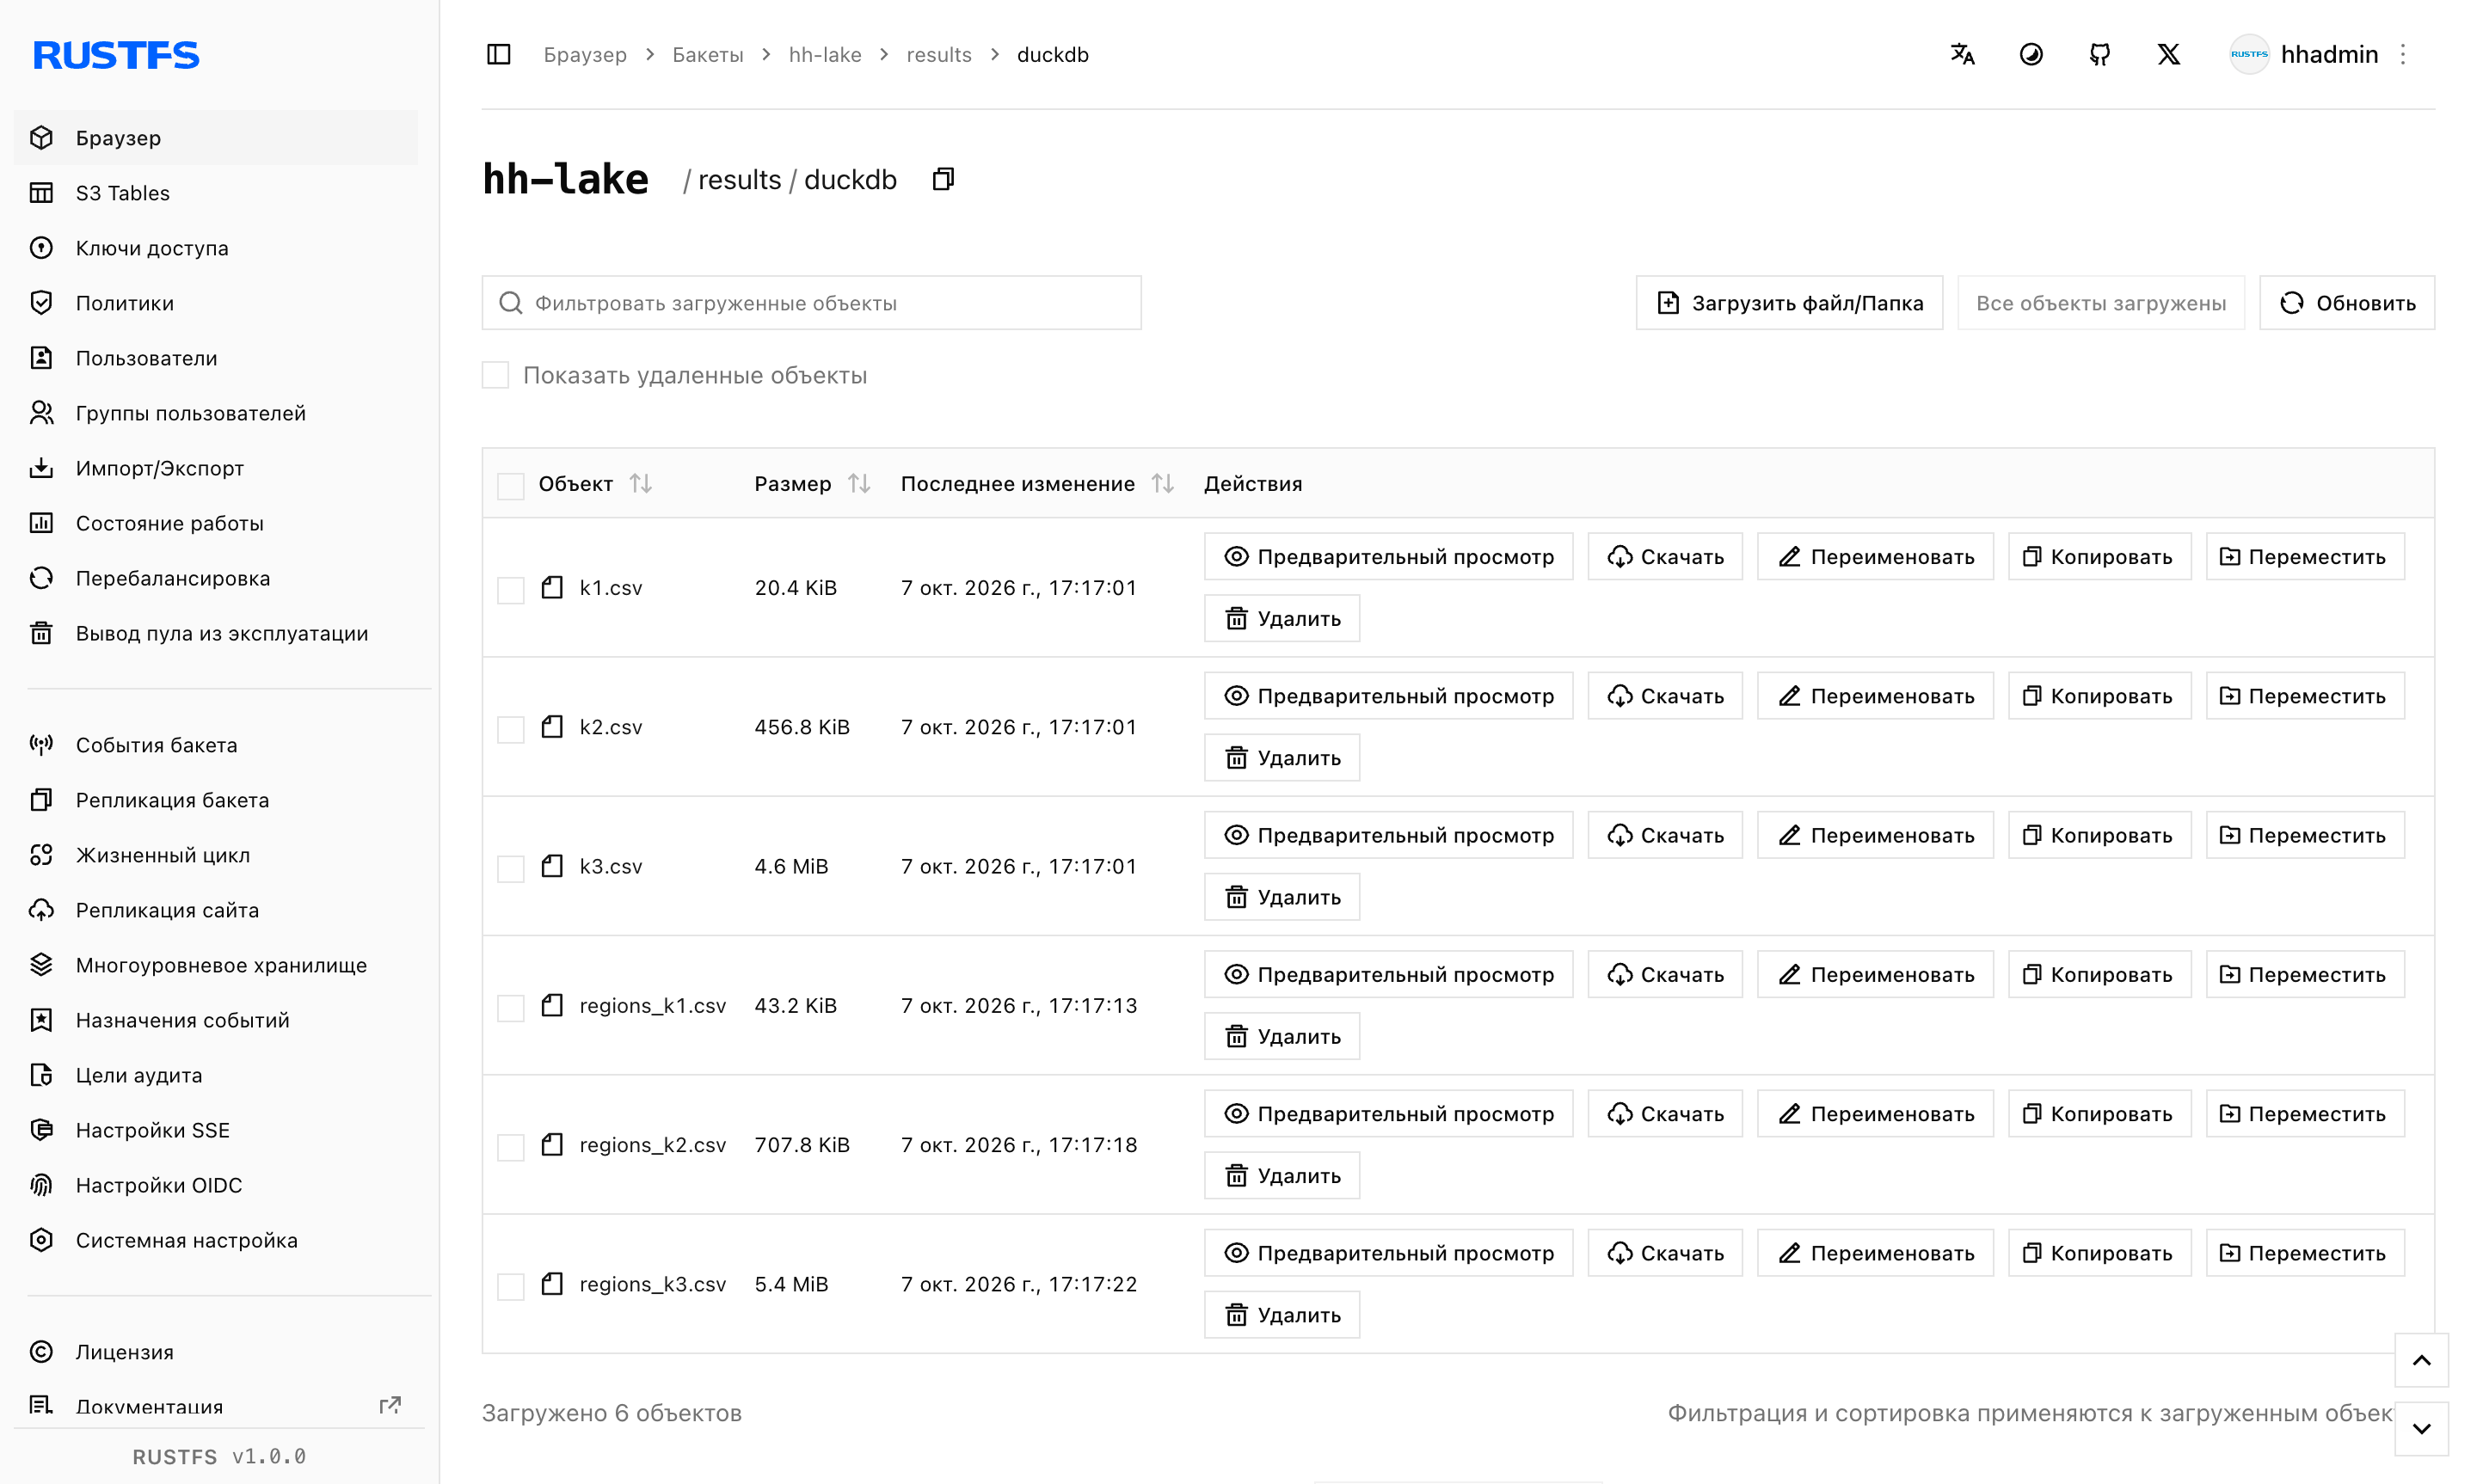
\includegraphics[width=0.49\linewidth]{img/console_duck.png}
  \caption{Результаты для трёх размеров стека в хранилище: \code{results/mapreduce/} и \code{results/duckdb/} (k1--k3 и региональные)}
\end{figure}

\subsection{Отказ маппера}
Маппер 7 на первой попытке завершается \code{os.\_exit(137)} --- настоящая смерть процесса, а не исключение. Пул ломается, мастер пересоздаёт его и перезапускает задачи; результат побайтно совпадает с прогоном без сбоя:
\begin{lstlisting}
$ uv run python -m hhlake.mr.run --k 1 2 3 --fail-mapper 7 --fail-attempt 1 --keep-tmp --job faulttest
map    task   7  attempt 1  @@crashed                  exit 137@@  pid 15532  1.87 s  failure 1 of 3
map    task   0  attempt 1  terminated (pool broken) exit -15  pid 15528  1.94 s  not charged
map    task   7  attempt 2  ++ok++   ...
s3://hh-lake/results/mapreduce/k1.csv  sha256 c071dfef...4bd73  object in S3 before this run: ++identical++
s3://hh-lake/results/mapreduce/k2.csv  sha256 ab85544b...19e3f  object in S3 before this run: ++identical++
s3://hh-lake/results/mapreduce/k3.csv  sha256 692ac358...0e8f960  object in S3 before this run: ++identical++
tmp kept: s3://hh-lake/tmp/mr/faulttest/  accepted 26 prefixes, 104 parts; orphans 2 prefixes (never read)
[2026-10-07 17:16:16 MSK] 120KiB map-7-a1/part-0      ~~<- мусор упавшей попытки~~
[2026-10-07 17:16:18 MSK] 120KiB map-7-a2/part-0..3   ~~<- принятая попытка (по манифесту)~~
\end{lstlisting}

\section{DuckDB: то же самое на SQL}

Условие варианта и нормализация написаны на SQL самостоятельно; DuckDB читает тот же объект из S3 через \code{httpfs} (\code{CREATE SECRET \dots ENDPOINT 'localhost:19000', URL\_STYLE 'path', USE\_SSL false}). Пары и тройки --- самосоединение по \code{vacancy\_id} с упорядочением навыков (порядок строк DuckDB совпадает с \code{sorted()} Python --- проверено на 19 пробах с кириллицей):
\begin{lstlisting}[language=SQL]
WITH vac AS (
    SELECT vacancy_id, area, key_skills
    FROM read_csv('s3://hh-lake/raw/it_vacancies_2024.csv', header = true, all_varchar = true)
    WHERE role = 'Программист, разработчик' AND name ILIKE '%php%'
),
skills AS (
    SELECT vacancy_id, area,
           list_sort(list_distinct(list_filter(
               list_transform(string_split(key_skills, ';'), x -> lower(trim(x))), x -> x <> ''))) AS skills
    FROM vac
),
s AS (SELECT vacancy_id, area, unnest(skills) AS skill FROM skills)
SELECT s1.skill AS skill1, s2.skill AS skill2, s3.skill AS skill3, count(*) AS count
FROM s AS s1
JOIN s AS s2 ON s2.vacancy_id = s1.vacancy_id AND s2.skill > s1.skill
JOIN s AS s3 ON s3.vacancy_id = s1.vacancy_id AND s3.skill > s2.skill
GROUP BY ALL ORDER BY count DESC, skill1, skill2, skill3
\end{lstlisting}
Доказательство чтения из хранилища --- статистика HTTP из \code{EXPLAIN ANALYZE}: весь объект скачан 27 Range-запросами:
\begin{lstlisting}
HTTPFS HTTP Stats   in: 808.3 MiB   #HEAD: 1   #GET: 27
GET body 847,619,384 B, ranges bytes=0-847619383, up to 32,000,000 B per GET, contiguous without overlap: True
\end{lstlisting}

\section{Верификация}

\code{hhlake.verify} читает оба набора из S3 и сравнивает их целиком (\code{EXCEPT ALL} в обе стороны):

\begin{table}[H]
\centering
\small
\caption{Контрольные числа MapReduce и DuckDB}
\footnotesize
\begin{tabular}{@{}clrrlrc@{}}
\toprule
$k$ & Способ & Ключей & $\Sigma$ count & Топ-1 & Частота & EXCEPT \\
\midrule
1 & MapReduce / DuckDB & 955 / 955 & 31\,835 / 31\,835 & php & 4\,033 / 4\,033 & 0 / 0 \\
2 & MapReduce / DuckDB & 15\,921 / 15\,921 & 135\,362 / 135\,362 & mysql + php & 2\,096 / 2\,096 & 0 / 0 \\
3 & MapReduce / DuckDB & 127\,466 / 127\,466 & 472\,071 / 472\,071 & git + mysql + php & 1\,030 / 1\,030 & 0 / 0 \\
\bottomrule
\end{tabular}
\end{table}
Итог \code{verdict: MATCH} для $k=1,2,3$, региональных наборов и наивной версии MapReduce. Дополнительно: при переименованном локальном CSV все 5 прогонов (MapReduce и DuckDB) завершились успешно --- данные берутся только из \code{hh-lake}.

\section{Рост числа сочетаний}

Вакансия с $n$ навыками даёт $\binom{n}{k}$ сочетаний, поэтому число эмитов растёт как $n^k/k!$:
\begin{table}[H]
\centering
\small
\caption{Рост числа сочетаний (4\,380 вакансий с навыками, в среднем 7,27 навыка, медиана 6, максимум 30)}
\begin{tabular}{@{}crrrrrr@{}}
\toprule
$k$ & $\Sigma\binom{n}{k}$ (эмитов) & На вакансию & После combiner & Уникальных ключей & Shuffle, Б & Результат, Б \\
\midrule
1 & 31\,835 & 7,3 & 4\,918 & 955 & 123\,425 & 20\,854 \\
2 & 135\,362 & 30,9 & 58\,813 & 15\,921 & 2\,090\,539 & 467\,629 \\
3 & 472\,071 & 107,8 & 334\,410 & 127\,466 & 15\,866\,064 & 4\,777\,942 \\
\bottomrule
\end{tabular}
\end{table}

Рост определяют «длинные» вакансии: среднее $\binom{n}{3}$ по вакансиям равно 107,8, а $\binom{7{,}27}{3}$ --- лишь 40. Вакансия с 30 навыками даёт $\binom{30}{3}=4\,060$ троек против $\binom{6}{3}=20$ у медианной; 69 вакансий с $n\ge20$ (1,6\,\%) дают 30\,\% всех троек. Combiner на $k=1$ сжимает эмиты в 6,5 раза, а на $k=3$ --- лишь в 1,4 раза: тройки редко повторяются внутри чанка, поэтому shuffle растёт в 128 раз от $k=1$ к $k=3$.

\begin{figure}[H]
  \centering
  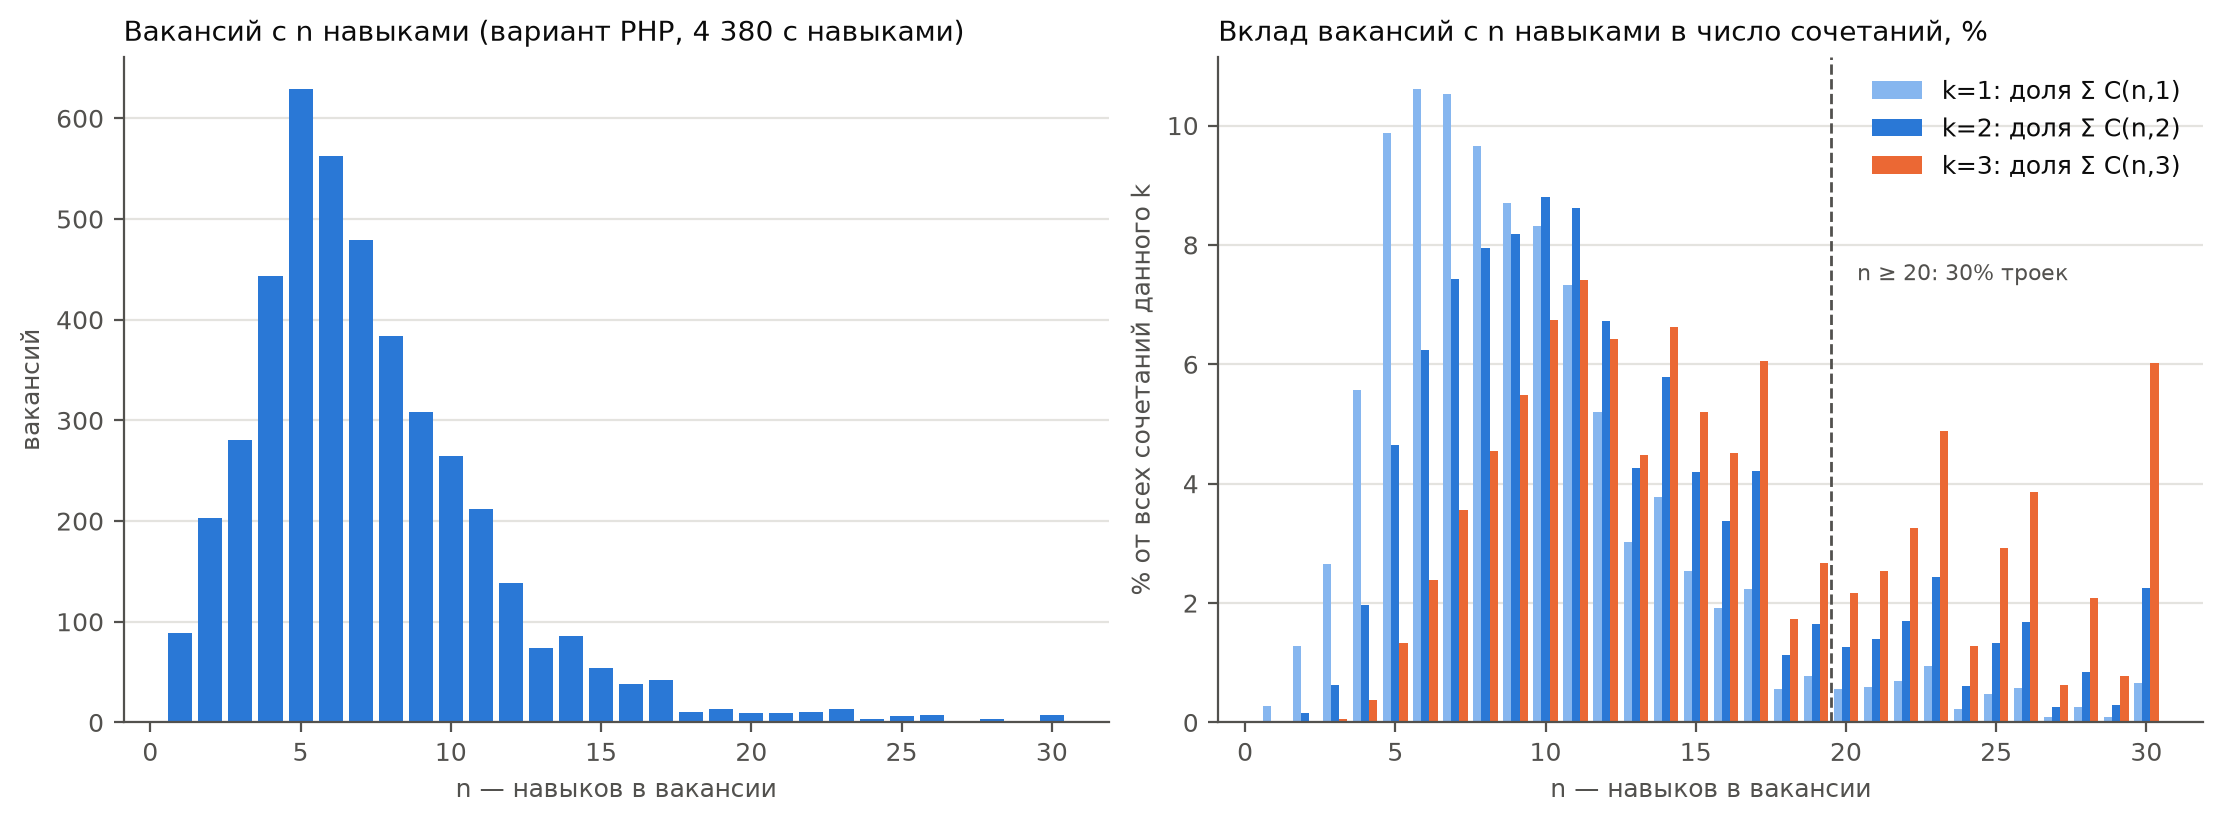
\includegraphics[width=0.95\linewidth]{img/growth.png}
  \caption{Распределение числа навыков и вклад вакансий в число сочетаний}
\end{figure}

\section{Профилирование: время и память}

Протокол: каждый сценарий --- отдельный процесс; перед сценарием RustFS перезапускается; 1 холодный прогон (не входит в статистику) и 5 тёплых. Память --- пик RSS \emph{суммы дерева процессов} (psutil, опрос 20 мс): для MapReduce это мастер и 10 воркеров. Сценарии запускаются с \code{--no-write}.

\begin{table}[H]
\centering
\small
\caption{MapReduce и DuckDB, тёплые прогоны (n = 5, mean $\pm$ std)}
\begin{tabular}{@{}lrrrrrr@{}}
\toprule
Сценарий & \multicolumn{2}{c}{MapReduce} & \multicolumn{2}{c}{DuckDB} & \multicolumn{2}{c}{MR / DuckDB} \\
\cmidrule(lr){2-3}\cmidrule(lr){4-5}\cmidrule(l){6-7}
 & время, с & пик, МиБ & время, с & пик, МиБ & время & память \\
\midrule
$k=1$ & 8,30 $\pm$ 1,24 & 1\,545 & 5,40 $\pm$ 0,18 & 412 & $\times$1,5 & $\times$3,8 \\
$k=2$ & 8,88 $\pm$ 1,31 & 1\,451 & 5,44 $\pm$ 0,11 & 428 & $\times$1,6 & $\times$3,4 \\
$k=3$ & 8,40 $\pm$ 0,58 & 1\,482 & 5,94 $\pm$ 0,44 & 483 & $\times$1,4 & $\times$3,1 \\
$k=1,2,3$ за проход & 8,59 $\pm$ 0,45 & 1\,378 & 5,46 $\pm$ 0,18 & 458 & $\times$1,6 & $\times$3,0 \\
\bottomrule
\end{tabular}
\end{table}

\begin{figure}[H]
  \centering
  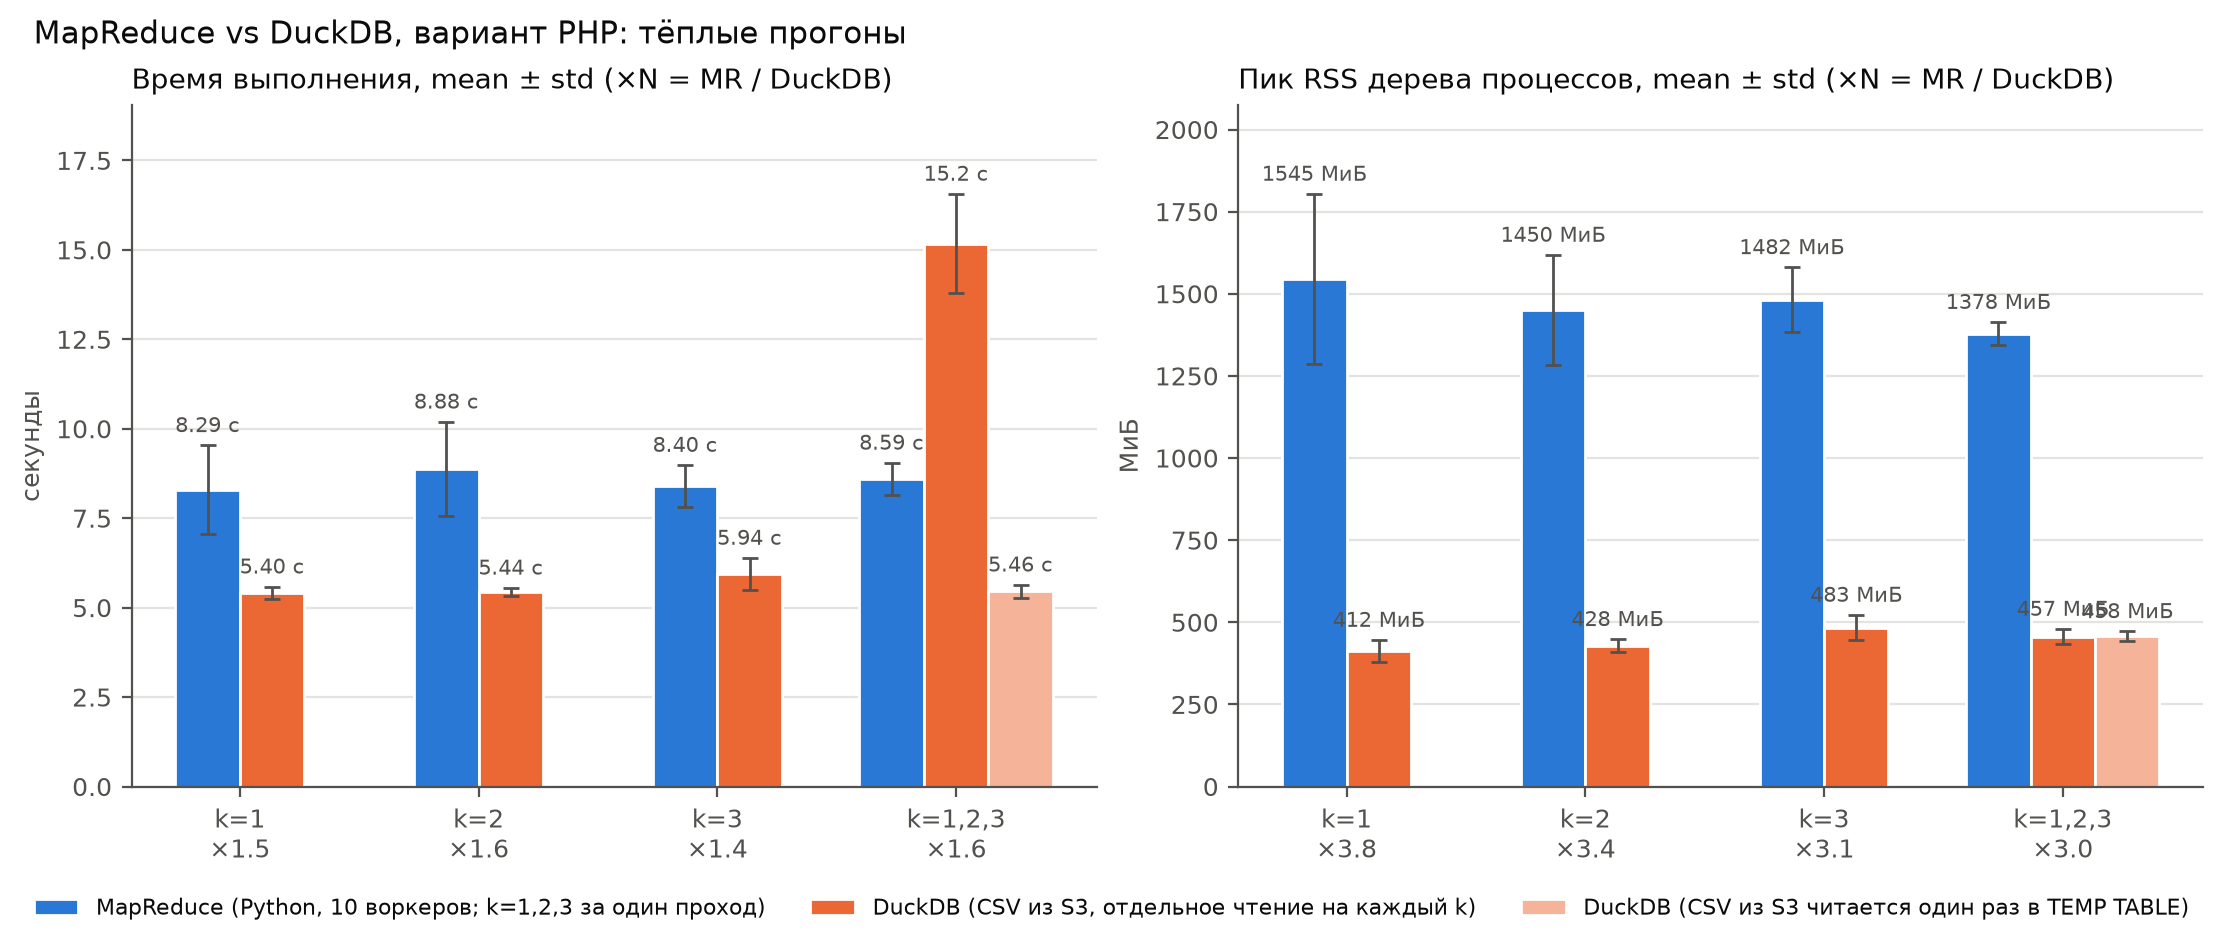
\includegraphics[width=\linewidth]{img/bench_main.png}
  \caption{Время и пик памяти по сценариям}
\end{figure}

\textbf{Почему так.}
\begin{itemize}
  \item \textbf{Время почти не зависит от $k$} (MapReduce 8,3--8,9\,с, DuckDB 5,4--5,9\,с): вариант --- лишь 2,3\,\% строк, а читать и разбирать приходится все 808 МиБ. В MapReduce 72,7\,\% времени задач --- Range GET и выравнивание, на сочетания и combiner уходит 0,9\,\%. Рост $k$ виден в shuffle (123 КБ $\to$ 15,9 МБ) и в памяти DuckDB (412 $\to$ 483 МиБ), но не во времени.
  \item \textbf{DuckDB быстрее в 1,5 раза и экономнее в 3--4 раза}: векторный C++-движок с параллельным CSV-reader в одном процессе, без сериализации и промежуточной записи. MapReduce --- 11 интерпретаторов Python (по 150--215 МиБ каждый: boto3 + буфер чанка 32 МиБ + Counter), shuffle через PUT/GET в S3 (104 + 104 запроса).
  \item \textbf{Масштабирование упирается в хранилище.} RustFS работает в Docker на той же машине и отдаёт одному таску около 21 МиБ/с, всем вместе --- около 140 МиБ/с. 1 $\to$ 4 воркера ускоряют лишь в 1,3 раза, дальше выигрыша нет, а память растёт почти линейно (436 $\to$ 1\,360 МиБ). Крупный чанк 128 МиБ лучше 32 МиБ: 11,3 против 15,5\,с (меньше запросов и shuffle-файлов) ценой 1,75 ГиБ памяти.
\end{itemize}

\begin{figure}[H]
  \centering
  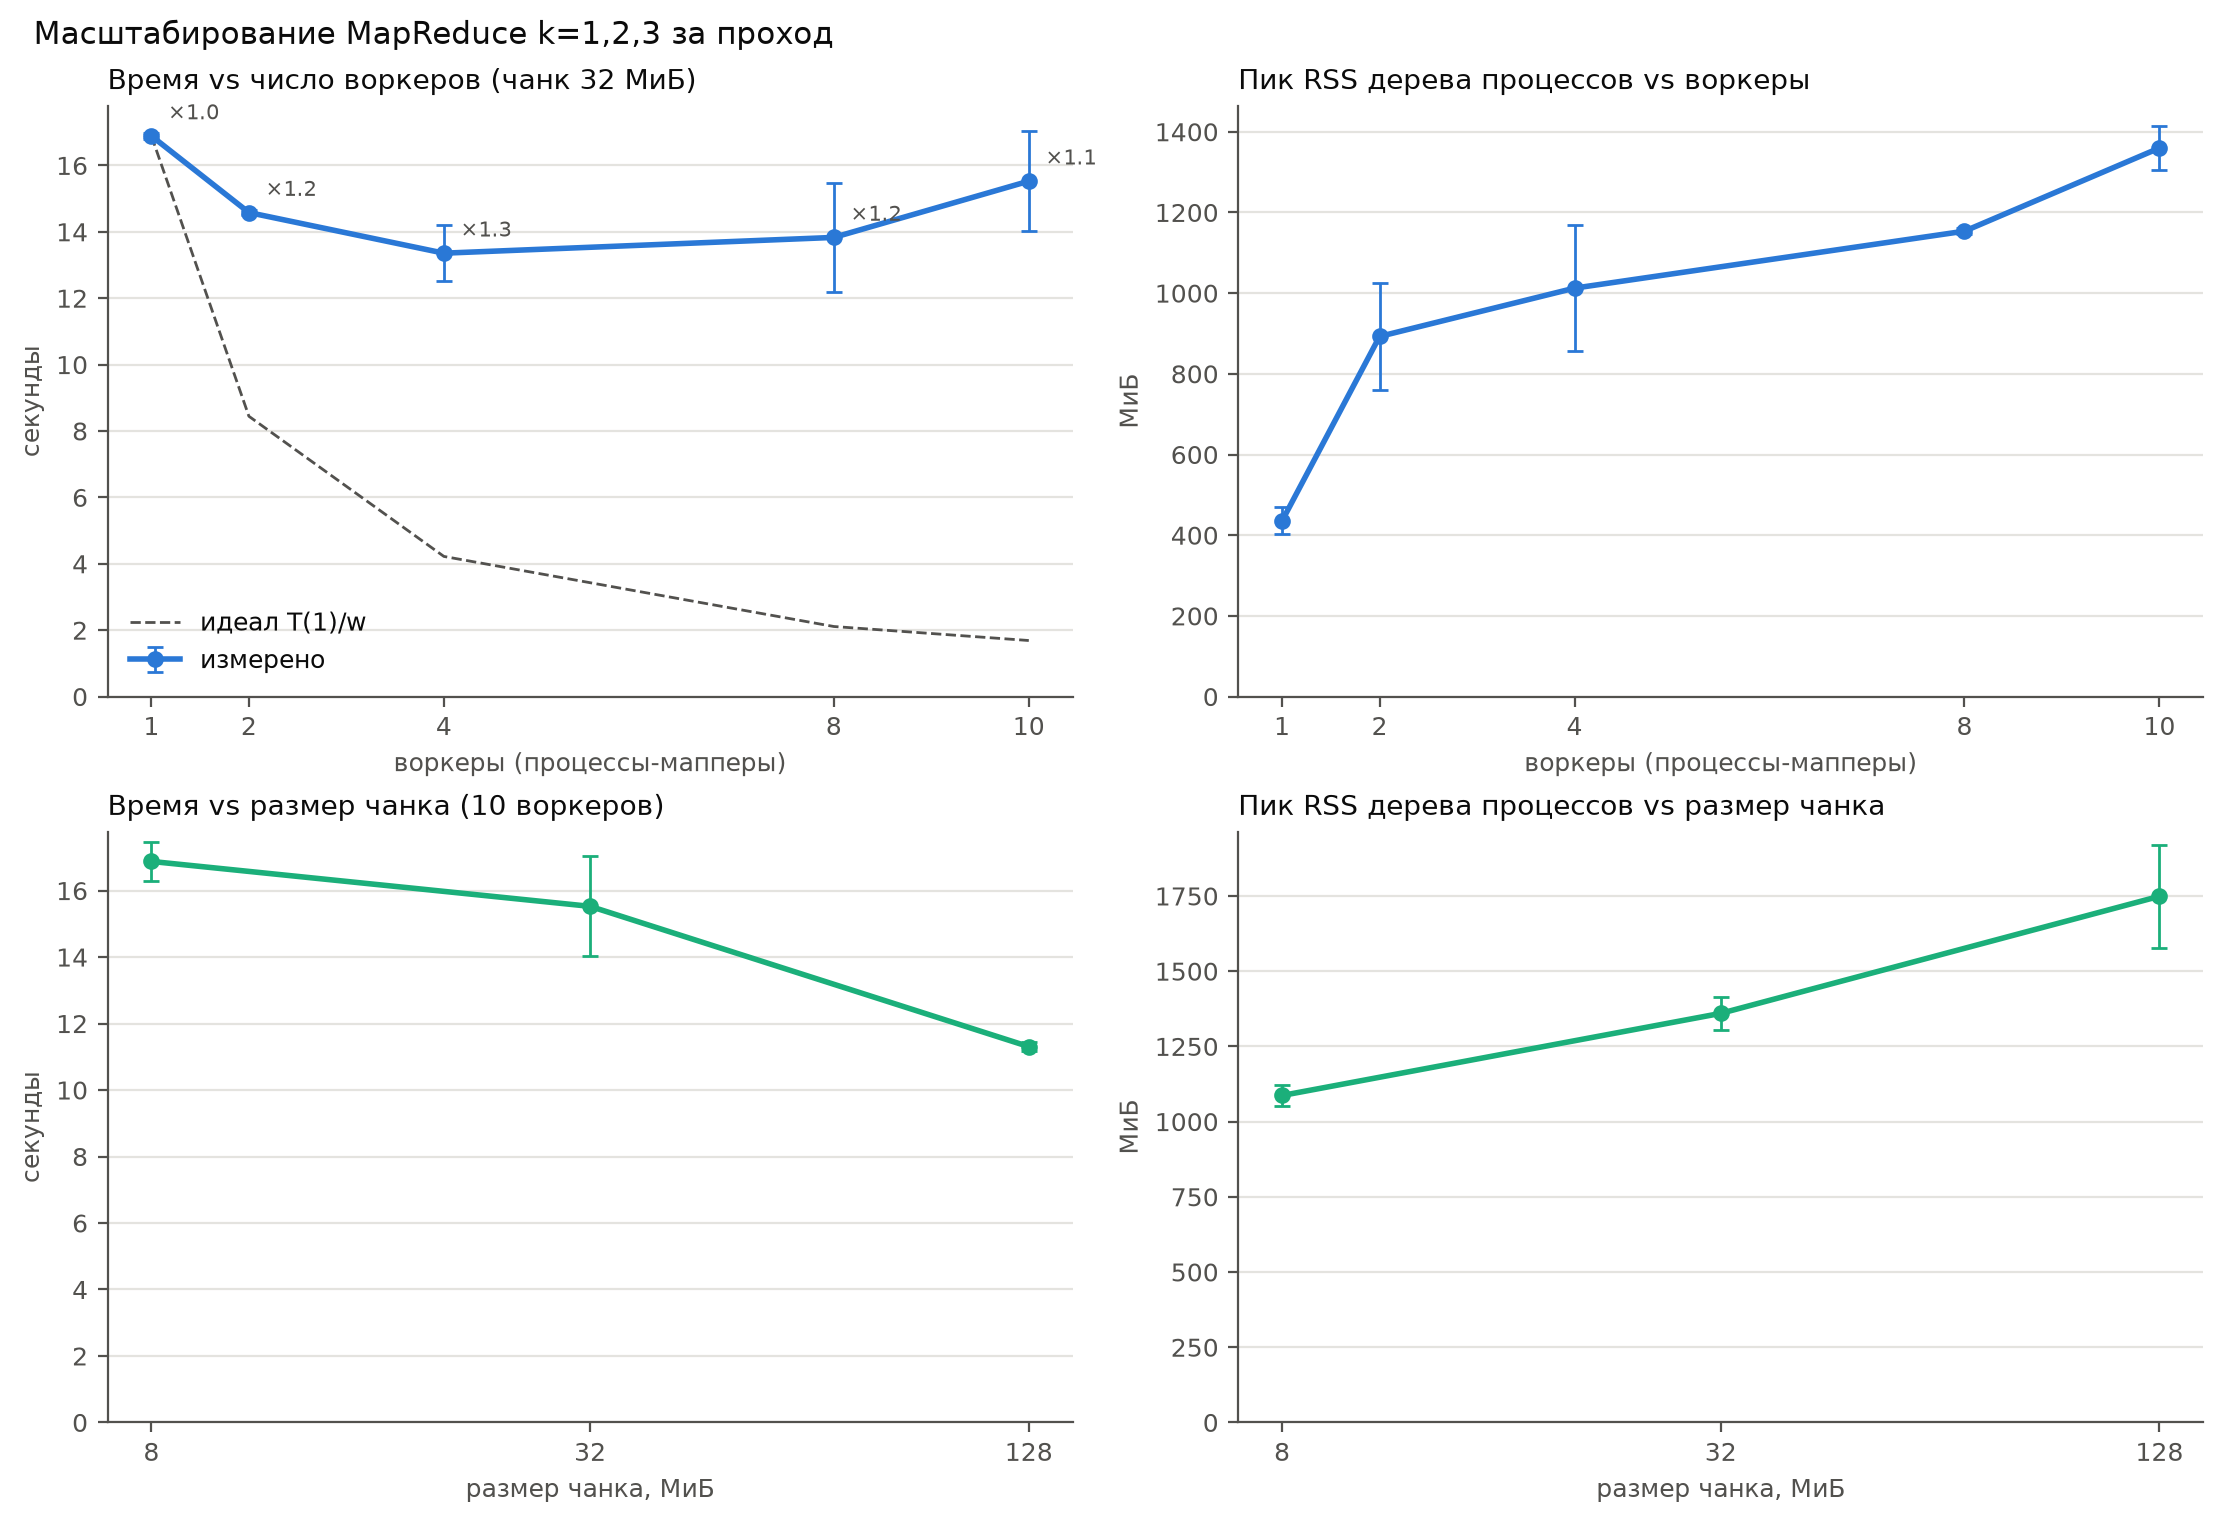
\includegraphics[width=0.82\linewidth]{img/bench_scaling.png}
  \caption{Масштабирование MapReduce по числу воркеров и размеру чанка (n = 3)}
\end{figure}

\subsection{Бонус: оптимизация «до» и «после»}

\begin{table}[H]
\centering
\small
\caption{Оптимизации (тёплые прогоны, n = 5)}
\begin{tabularx}{\linewidth}{@{}>{\raggedright\arraybackslash}p{4.3cm}rrrrL@{}}
\toprule
Что & \multicolumn{2}{c}{До} & \multicolumn{2}{c}{После} & Причина \\
\cmidrule(lr){2-3}\cmidrule(lr){4-5}
 & с & МиБ & с & МиБ & \\
\midrule
DuckDB: CSV $\to$ Parquet (zstd) & 14,10 & 457 & \textbf{1,47} & 318 & $\times$9,6: читаются только 5 нужных колонок, объект в 5 раз меньше (162 МиБ), нет разбора CSV \\
DuckDB: 3 скана $\to$ 1 скан (TEMP TABLE) & 15,17 & 457 & \textbf{5,46} & 458 & $\times$2,8: CSV из S3 читается один раз для всех $k$ \\
MapReduce: чанк 32 $\to$ 128 МиБ & 15,53 & 1\,360 & \textbf{11,31} & 1\,749 & $\times$1,4: 7 задач вместо 26, меньше запросов и shuffle-объектов \\
MapReduce v1 (1 процесс, без combiner) $\to$ v2 (10 воркеров) & \textbf{4,42} & 183 & 8,67 & 1\,426 & ускорения нет: один потоковый GET быстрее 26 параллельных Range GET к локальному RustFS; накладные расходы процессов и shuffle превышают выигрыш \\
\bottomrule
\end{tabularx}
\end{table}
Главный вывод бонуса: на этом объёме узкое место --- ввод-вывод, а не вычисления. Поэтому помогает уменьшение объёма читаемых данных (Parquet, один скан), а параллелизм MapReduce на одной машине с локальным хранилищем не окупается. На кластере, где диски и узлы независимы, картина была бы обратной.

\section{Навыки и зарплата}

Зарплата: только RUR; середина вилки (или одна граница); gross $\times$\,0,87; отсечение вне 20\,000--1\,000\,000. Таких вакансий 3\,055 (медиана 140\,000\,руб.), с зарплатой и навыками --- 2\,569. Прибавка пары $(A,B)$ считается от медианы \textbf{более частого} навыка $A$ (по \code{results/mapreduce/k1.csv}); прибавка тройки --- от \textbf{самой частой пары} внутри неё (по \code{k2.csv}). Порог: $n\ge30$ вакансий с зарплатой и $\ge10$ работодателей (469 пар, 1\,021 тройка).

\begin{table}[H]
\centering
\scriptsize
\setlength{\tabcolsep}{3pt}
\caption{Пары: наибольшее повышение и понижение медианной зарплаты, руб. ($\Delta$ --- прибавка к медиане базы)}
\begin{tabular}{@{}llrrrrr|llrrrrr@{}}
\toprule
\multicolumn{7}{c|}{\textcolor{ok}{\textbf{Повышают}}} & \multicolumn{7}{c}{\textcolor{bad}{\textbf{Понижают}}} \\
База & + навык & $n$ & мед. & $n_{\text{б}}$ & мед. базы & $\Delta$ & База & + навык & $n$ & мед. & $n_{\text{б}}$ & мед. базы & $\Delta$ \\
\midrule
sql & rabbitmq & 44 & 262\,500 & 505 & 130\,000 & +132\,500 & postgresql & jquery & 30 & 104\,400 & 567 & 170\,000 & $-$65\,600 \\
php & highload & 31 & 261\,000 & 2\,362 & 140\,000 & +121\,000 & docker & css & 42 & 110\,000 & 570 & 175\,000 & $-$65\,000 \\
ооп & solid & 35 & 250\,000 & 507 & 130\,000 & +120\,000 & docker & html & 55 & 115\,000 & 570 & 175\,000 & $-$60\,000 \\
api & php7 & 47 & 250\,000 & 356 & 145\,000 & +105\,000 & php & адм. сайтов & 34 & 80\,000 & 2\,362 & 140\,000 & $-$60\,000 \\
php & golang & 31 & 240\,000 & 2\,362 & 140\,000 & +100\,000 & symfony & html & 56 & 128\,075 & 417 & 180\,000 & $-$51\,925 \\
linux & rabbitmq & 54 & 250\,000 & 375 & 155\,000 & +95\,000 & php & wordpress & 130 & 90\,000 & 2\,362 & 140\,000 & $-$50\,000 \\
\bottomrule
\end{tabular}
\end{table}

\begin{table}[H]
\centering
\scriptsize
\setlength{\tabcolsep}{3pt}
\caption{Тройки: база --- самая частая пара внутри тройки, руб.}
\begin{tabular}{@{}llrrrr|llrrrr@{}}
\toprule
\multicolumn{6}{c|}{\textcolor{ok}{\textbf{Повышают}}} & \multicolumn{6}{c}{\textcolor{bad}{\textbf{Понижают}}} \\
Базовая пара & + навык & $n$ & мед. & мед. базы & прибавка & Базовая пара & + навык & $n$ & мед. & мед. базы & прибавка \\
\midrule
php + sql & rabbitmq & 44 & 262\,500 & 130\,500 & +132\,000 & docker + postgresql & javascript & 32 & 120\,900 & 200\,000 & $-$79\,100 \\
php + ооп & solid & 35 & 250\,000 & 130\,000 & +120\,000 & docker + php & css & 39 & 105\,000 & 175\,000 & $-$70\,000 \\
api + mysql & php7 & 38 & 262\,500 & 145\,000 & +117\,500 & docker + php & html & 52 & 111\,875 & 175\,000 & $-$63\,125 \\
api + sql & backend & 37 & 262\,500 & 150\,000 & +112\,500 & php + symfony & html & 55 & 126\,150 & 180\,000 & $-$53\,850 \\
mysql + postgresql & rabbitmq & 76 & 261\,750 & 160\,000 & +101\,750 & mysql + php & wordpress & 67 & 90\,000 & 140\,000 & $-$50\,000 \\
\bottomrule
\end{tabular}
\end{table}

\textbf{Интерпретация.} Зарплату \textbf{повышают} навыки серверной архитектуры и нагрузки: rabbitmq (медиана 215\,000), highload (250\,000), golang (232\,500), solid, kafka, clickhouse --- это вакансии бэкенда высоконагруженных сервисов, где PHP --- один из языков, а не весь стек. \textbf{Понижают} вёрстка и CMS: html и css (медиана по 100\,000), jquery, wordpress (92\,500), «администрирование сайтов» (80\,000) --- это поддержка сайтов и фулстек в веб-студиях, где PHP-разработчик совмещает вёрстку. Устаревшая версия языка тоже маркер более дешёвых вакансий: php5 --- 100\,000 против php7 155\,000. Оговорка: часть вакансий --- перепубликации одного работодателя, поэтому введён порог по числу работодателей.

\section{Региональный анализ}

Выбраны Москва, Санкт-Петербург и Екатеринбург (у Екатеринбурга 146 вакансий с зарплатой против 111 у Новосибирска). Профиль считается DuckDB по S3, частоты навыков, пар и троек берутся из MapReduce (\code{results/mapreduce/regions\_k\{1,2,3\}.csv}), медианы --- DuckDB:
\begin{lstlisting}[language=Python]
    WITH scoped AS (
        SELECT area AS scope, * FROM vac WHERE {duck.REGION_FILTER}
        UNION ALL
        SELECT {duck.quote(ALL)} AS scope, * FROM vac
    )
    SELECT
        scope AS area,
        count(*) AS vacancies,
        count(*) FILTER (WHERE len(skills) > 0) AS with_skills,
        count(net) AS with_salary,
        quantile_cont(net, 0.25) AS q1,
        median(net) AS median,
        quantile_cont(net, 0.75) AS q3,
        avg(CAST(schedule = {duck.quote(REMOTE)} AS INT)) AS remote_share,
        {experience},
        count(DISTINCT employer_id) AS employers,
        {subsets}
    FROM scoped
    GROUP BY scope
\end{lstlisting}
Здесь \code{vac} --- вакансии варианта из S3 с нормализованными навыками и зарплатой \code{net}, \code{\{subsets\}} --- медианы по опыту и формату работы (\code{median(net) FILTER (WHERE \dots)}). Фрагмент из \code{src/hhlake/regions.py}, сокращён на две строки с долями.

\begin{table}[H]
\centering
\footnotesize
\caption{Таблица 1. Профиль региона (зарплата на руки, руб.)}
\begin{tabular}{@{}lrrrr@{}}
\toprule
Показатель & Москва & Санкт-Петербург & Екатеринбург & Весь вариант \\
\midrule
Вакансий / с навыками & 2\,127 / 1\,692 & 790 / 646 & 205 / 169 & 5\,382 / 4\,380 \\
С зарплатой (доля) & 1\,022 (48,0\,\%) & 479 (60,6\,\%) & 146 (71,2\,\%) & 3\,055 (56,8\,\%) \\
Q1 / \textbf{медиана} / Q3 & 130 / \textbf{174} / 225 тыс. & 104 / \textbf{150} / 200 тыс. & 90 / \textbf{125} / 175 тыс. & 95 / \textbf{140} / 185 тыс. \\
Медиана: опыт 1--3 / 3--6 лет & 140 / 200 тыс. & 120 / 175 тыс. & 120 / 144 тыс. & 115 / 175 тыс. \\
Удалённая работа (доля) & 51,8\,\% & 40,8\,\% & 31,2\,\% & 42,1\,\% \\
Медиана: удалёнка / офис & 180 / 163 тыс. & 150 / 149 тыс. & 140 / 125 тыс. & 150 / 130 тыс. \\
Опыт 3+ лет (доля вакансий) & 64,1\,\% & 51,1\,\% & 34,6\,\% & 49,0\,\% \\
Работодателей & 1\,013 & 414 & 123 & 2\,248 \\
\bottomrule
\end{tabular}
\end{table}

\begin{table}[H]
\centering
\scriptsize
\setlength{\tabcolsep}{3pt}
\caption{Таблица 2. Топ-3 навыков, пар и троек по регионам: частота (MapReduce), доля вакансий с навыками, медиана зарплаты (DuckDB)}
\begin{tabular}{@{}clrr|lrr|lrr@{}}
\toprule
 & \multicolumn{3}{c|}{Москва} & \multicolumn{3}{c|}{Санкт-Петербург} & \multicolumn{3}{c}{Екатеринбург} \\
$k$ & сочетание & частота & медиана & сочетание & частота & медиана & сочетание & частота & медиана \\
\midrule
1 & php & 1\,548 (92\,\%) & 175\,000 & php & 602 (93\,\%) & 150\,000 & php & 156 (92\,\%) & 130\,500 \\
1 & mysql & 834 (49\,\%) & 167\,475 & mysql & 359 (56\,\%) & 150\,000 & mysql & 101 (60\,\%) & 125\,000 \\
1 & git & 671 (40\,\%) & 170\,000 & git & 263 (41\,\%) & 145\,000 & javascript & 53 (31\,\%) & 100\,000 \\
\midrule
2 & mysql+php & 749 (44\,\%) & 169\,650 & mysql+php & 344 (53\,\%) & 150\,000 & mysql+php & 94 (56\,\%) & 125\,000 \\
2 & git+php & 618 (37\,\%) & 172\,000 & git+php & 249 (39\,\%) & 145\,000 & javascript+php & 47 (28\,\%) & 95\,000 \\
2 & laravel+php & 498 (29\,\%) & 160\,950 & laravel+php & 222 (34\,\%) & 148\,770 & git+php & 44 (26\,\%) & 120\,000 \\
\midrule
3 & git+mysql+php & 368 (22\,\%) & 160\,950 & git+mysql+php & 165 (26\,\%) & 140\,000 & html+mysql+php & 35 (21\,\%) & 125\,000 \\
3 & laravel+mysql+php & 250 (15\,\%) & 160\,000 & laravel+mysql+php & 129 (20\,\%) & 142\,500 & javascript+mysql+php & 34 (20\,\%) & 95\,000 \\
3 & git+laravel+php & 217 (13\,\%) & 160\,000 & javascript+mysql+php & 116 (18\,\%) & 121\,800 & css+mysql+php & 30 (18\,\%) & 125\,000 \\
\bottomrule
\end{tabular}
\end{table}

\textbf{Наблюдения.}
\begin{enumerate}
  \item \textbf{Москва платит больше даже при том же опыте.} Медиана выше Петербурга на 16\,\% и Екатеринбурга на 39\,\%; первый квартиль Москвы (130 тыс.) выше медианы Екатеринбурга. При опыте 1--3 года разрыв Москвы с обоими городами --- 17\,\%, при 3--6 годах с Екатеринбургом --- 39\,\%. Часть разрыва объясняет и структура спроса: в Москве 64\,\% вакансий требуют 3+ лет опыта, в Екатеринбурге --- 35\,\%.
  \item \textbf{Москва реже показывает зарплату}: вилка есть у 48\,\% вакансий против 71\,\% в Екатеринбурге, поэтому московская медиана посчитана по менее представительной выборке.
  \item \textbf{Удалёнка в регионах оплачивается по более высокой вилке}: в Екатеринбурге удалённые вакансии на 12\,\% дороже офисных (140 против 125 тыс.), в Петербурге разницы нет --- удалённо регионы конкурируют за кандидатов со столичными работодателями.
  \item \textbf{Разный стек.} В Москве и Петербурге чаще symfony (23,5\,\% и 27,1\,\% против 12,4\,\%) и postgresql; самая дорогая тройка московского топа --- docker+php+postgresql (225 тыс.). В Екатеринбурге больше вёрстки: html у 26\,\% вакансий против 15,8\,\% в Москве, css --- 21,3\,\% против 11,1\,\%; все топ-тройки Екатеринбурга содержат html, css или javascript, и их медианы (95--125 тыс.) согласуются с выводом раздела 7: вёрстка понижает зарплату.
\end{enumerate}

\begin{keybox}
\textbf{Итог.} MapReduce, читающий объект из \code{hh-lake} Range-запросами, и SQL в DuckDB дали идентичные частоты навыков, пар и троек (955 / 15\,921 / 127\,466 ключей, расхождений 0); отказ маппера не меняет результат. На одной машине DuckDB быстрее в 1,5 раза и требует в 3--4 раза меньше памяти, а наибольший выигрыш даёт уменьшение объёма чтения (Parquet: $\times$9,6). Для PHP-разработчика зарплату поднимают навыки высоконагруженного бэкенда (RabbitMQ, Highload, Go, SOLID: до +130 тыс.), а опускают вёрстка и CMS (HTML/CSS, jQuery, WordPress: до $-$65 тыс.).
\end{keybox}

\end{document}
